\section{Langages intermédiaires}

Le langage C \cite{KandR,AnsiC} a été conçu pour être une sorte d'assembleur
portable, permettant décrire du code indépendamment de l'architecture sur
laquelle il sera compilé. Historiquement, c'est il a permis de créer Unix, et
ainsi de nombreux logiciels bas niveau sont écrits en C. En particulier, il
existe des compilateurs de C vers les différents langages machine pour à peu
près toutes les architectures.

Lors de l'écriture d'un compilateur, on a besoin d'un langage intermédiaire qui
fasse l'intermédiaire entre \emph{frontend} et \emph{backend}. Avec ce langage,
on doit pouvoir (facilement) réaliser les types d'opérations suivantes :

\begin{itemize}
\item
  compiler ce langage vers un langage machine (interface avec le
  \emph{backend}).
\item
  exprimer des transformations intermédiaires sur cette représentation
  (analyses sémantiques, optimisations, etc).
\end{itemize}

À cause du premier point, un langage comme C est très séduisant, mais
malheureusement il a de nombreux défauts qui font qu'il ne remplit pas le
deuxième. Par exemple, certaines instructions sont ambiguës, et l'ensemble des
opération n'est pas orthogonal (on peut faire la même chose de plusieurs
manières).

Pour pallier ce problème, une première solution peut être d'ajouter des
contraintes au C intermédiaire manipulé pour en obtenir un sous-langage. De
nombreux sous-ensembles ont été définis pour aller dans ce sens.

\subsubsection{Critères}

Les critères à évaluer sont les suivants :

\paragraph{Forme (textuel / langage d'implem)}

Quelle est la représentation du langage ? Est-ce une bibliothèque (si oui, dans
quel langage) a-t'il une forme textuelle (si oui, pour quels langages des
\emph{parsers} existent ils).

\paragraph{Maturité}

\paragraph{Tools}

\paragraph{Support}

Le langage a-t'il ``fait ses preuves'' ? Est-il susceptible de changer ?

\paragraph{Scope (analyse / compil)}

Pour quel type d'utilisation a-t'il été conçu ?

\paragraph{Expressivité}

Peut-on compiler ``tout C'' ?

\paragraph{Orthogonalité}

\paragraph{Typage}

\subsubsection{Langages}

\paragraph{LLVM}

LLVM\cite{llvm-pres} est un backend de compilateur développé par Apple.

\paragraph{Cmm (Haskell)}

\paragraph{Cmm (OCaml)}

\paragraph{CIL}

\paragraph{Clight}

\paragraph{Cminor}

\paragraph{Cminusminus}

\cite{spjcmm}

http://www.cminusminus.org/

\paragraph{Newspeak}

\section{Newspeak}

\section{Chaîne de compilation}

\begin{figure}
  \begin{tikzpicture}\shorthandoff{!}
\tikzstyle{file}=[draw, shape=rectangle, node distance=2.2cm, minimum
height=1cm, shade, top color=white,
    bottom color=blue!50!black!20, draw=blue!40!black!60, very thick];

\node [file] (c1) {\textcolor{black}{.c}};
\node [file, below of=c1] (c2) {\textcolor{black}{.c}};
\node [node distance=2.2cm, below of=c2] (c3) {};

\node [file, minimum height=0, node distance=5mm, above of=c3,draw] (c3b) {.adb};
\node [file, minimum height=0, node distance=5mm, below of=c3,draw] (c3s) {.ads};

\path (c3b.north west) ++(-3mm,3mm) [draw,dotted] rectangle ($(c3s.south east)+(3mm,-3mm)$);

\node [below of=c3, node distance=2.2cm] (c4){};

\node [file, right of=c1] (cc1) {\textcolor{black}{.c}};
\node [file, right of=c2] (cc2) {\textcolor{black}{.c}};
\node [node distance=2.2cm, right of=c3] (cc3) {};

\node [below of=cc3, node distance=2.2cm](cc4){};

\draw[->] (c1) -- node[above] {{\tiny \ttfamily cpp}} (cc1);
\draw[->] (c2) -- (cc2);

\node [file, right of=cc1] (no1) {\textcolor{black}{.no}};
\node [file, right of=cc2] (no2) {\textcolor{black}{.no}};
\node [file, right of=cc3] (no3) {\textcolor{black}{.no}};

\node [below of=no3, node distance=2.2cm](no4){};

\draw[->] (cc1) -- node[above] {{\tiny \ttfamily c2newspeak -c}} (no1);
\draw[->] (cc2) --  (no2);

\draw[->] ($ (c3b.north east)!0.5!(c3s.south east) + (3mm,0) $) -- node[above] {\tiny \ttfamily ada2newspeak -c} (no3);


\node [file, right of=no2] (npk) {\textcolor{black}{.npk}};

\node [right of=no3, node distance=2.2cm](npk2){};
\node [right of=no4, node distance=2.2cm](npk3){};

\node[draw, ellipse, right of=no2, minimum height=3cm]{};

\draw[->] (no1) -- node {} (npk);
\draw[->] (no2) -- node[above] {{\tiny \ttfamily c2newspeak}} (npk);
\draw[->] (no3) -- node {} (npk);


\node [file, right of=npk, node distance=3cm, yshift=1cm](warn)
    {\textcolor{black}{\parbox{2cm}{\centering Programme \linebreak typé}}};
\node [right of=npk, node distance=3cm, yshift=-1cm](warnn)
    {\textcolor{black}{Erreurs}};

\node [right of=npk3, node distance=3cm](analyser2){};

\node [right of=npk, node distance=3cm] {\small ou};

\draw[->] (npk) -- node[above, yshift=2mm] {{\tiny \ttfamily ptrtype}} (warn);

\draw[->] (npk) -- (warnn);

\draw[->] (c4)   -- node[above, text depth=3pt] {\footnotesize Pr\'etraitement} (cc4);
\draw[->] (cc4)  -- node[above, text depth=3pt] {\footnotesize Compilation} (no4);
\draw[->] (no4)  -- node[above, text depth=3pt] {\footnotesize \'Edition de liens} (npk3);
\draw[->] (npk3) -- node[above, text depth=3pt] {\footnotesize Analyse} (analyser2);
\end{tikzpicture}

  \caption{Compilation depuis Newspeak}
  \label{fig:compil-npk}
\end{figure}

La compilation vers C est faite en trois étapes (figure~\ref{fig:compil-npk}) :
prétraitement du code source, compilation de C prétraité vers \newspeak{}, puis
compilation de \newspeak{} vers ce langage.

\subsection{Prétraitement}

\ctonewspeak{} travaillant uniquement sur du code prétraité (dans directives de
préprocesseur), la première étape consiste donc à faire passer le code par \cpp.

\subsection{Compilation (levée des ambigüités)}

Cette passe est réalisée par l'utilitaire \ctonewspeak{}. L'essentiel de la
compilation consiste à mettre à plat les définition de types, et à simplifier le
flôt de contrôle. C en effet propose de nombreuses constructions ambigües ou
redondantes.

Au contraire, \newspeak{} propose un nombre réduit de constructions. Rappelons
que le but de ce langage est de faciliter l'analyse statique : des constructions
orthogonales permettent donc d'éviter la duplication de règles sémantique, ou de
code lors de l'implémentation d'un analyseur.

Par exemple, plutôt que de fournir une boucle while, une boucle do/while et une
boucle for, \newspeak{} fournit une unique boucle \npkWhile{}. La sortie de
boucle est compilée vers un \npkGoto{}, qui est toujours un saut vers l'avant
(similaire à un "break" généralisé).

La sémantique de \newspeak{} et la traduction de C vers \newspeak{} sont
décrites dans \cite{newspeak}. En ce qui concerne l'élimination des sauts vers
l'arrière, on peut se référer à \cite{goto}.

\subsection{Annotations}

\newspeak{} a de nombreux avantages, mais pour une analyse par typage il est
trop bas niveau. Par exemple, dans le code suivant

\begin{Verbatim}[commandchars=\\\{\}]
\PY{k}{struct} \PY{n}{s} \PY{p}{\PYZob{}}
    \PY{k+kt}{int} \PY{n}{a}\PY{p}{;}
    \PY{k+kt}{int} \PY{n}{b}\PY{p}{;}
\PY{p}{\PYZcb{}}\PY{p}{;}

\PY{k+kt}{int} \PY{n+nf}{main}\PY{p}{(}\PY{k+kt}{void}\PY{p}{)}
\PY{p}{\PYZob{}}
    \PY{k}{struct} \PY{n}{s} \PY{n}{x}\PY{p}{;}
    \PY{k+kt}{int} \PY{n}{y}\PY{p}{[}\PY{l+m+mi}{10}\PY{p}{]}\PY{p}{;}
    \PY{n}{x}\PY{p}{.}\PY{n}{b} \PY{o}{=} \PY{l+m+mi}{1}\PY{p}{;}
    \PY{n}{y}\PY{p}{[}\PY{l+m+mi}{1}\PY{p}{]} \PY{o}{=} \PY{l+m+mi}{1}\PY{p}{;}
    \PY{k}{return} \PY{l+m+mi}{0}\PY{p}{;}
\PY{p}{\PYZcb{}}
\end{Verbatim}


\subsection{Implantation de l'algorithme de typage}

L'inférence de types se fait par unification. Commençons par étudier le cas du
lambda-calcul simplement typé.

\newcommand{\gramisa}[0]{::=}
\newcommand{\gramor}[0]{|\hspace{3mm}}

\paragraph{Termes}

\begin{align*}
  t \gramisa & x       & \textrm{Variable} \\
    \gramor  & λ x . t & \textrm{Abstraction} \\
    \gramor  & t       & \textrm{Application} \\
    \gramor  & n       & \textrm{Entier}
\end{align*}

\paragraph{Types}

\begin{align*}
  τ \gramisa &  \tInt          & \textrm{Entier}\\
    \gramor  & τ \rightarrow τ & \textrm{Fonction}
\end{align*}

\paragraph{Contextes}

\begin{align*}
  Γ \gramisa & ε     & \textrm{Contexte vide}\\
    \gramor  & Γ,x:τ & \textrm{Extension}
\end{align*}

\paragraph{Règles}

\begin{align*}
\irule{Int}{ }{Γ⊢n:\tInt}
&&
\irule{Var}{x∈Γ \\ τ=Γ(x)}{Γ⊢x:τ}
\\
\irule{App}{Γ⊢f:τ_1 \rightarrow τ_2 \\ Γ ⊢ x : τ_1}{Γ ⊢ f x : τ_2}
&&
\irule{Abs}{Γ,x:τ_1⊢ y : τ_2}{Γ⊢ λx.y:τ_1 \rightarrow τ_2}
\end{align*}

\begin{center}\rule{3in}{0.4pt}\end{center}

L'inférence de types se fait par unification, en suivant les règles de typage.

\insertcode{ex-unif-c.c}

\insertcode{ex-unif-tpk.ml}

\begin{figure}

  \subfloat[][]{
  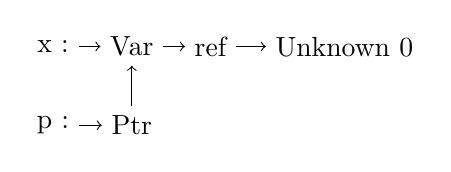
\begin{tikzpicture}
  \node               (var) {Var};
  \node[right of=var] (ref) {ref};
  \node[right of=ref, node distance=1.7cm] (u0) {Unknown 0};
  \node[below of=var] (ptr) {Ptr};
  \node[left of=var]  (x) {x :};
  \node[left of=ptr] (p) {p :};
  \draw[->] (x) -- (var);
  \draw[->] (p) -- (ptr);
  \draw[->] (ptr) -- (var);
  \draw[->] (var) -- (ref);
  \draw[->] (ref) -- (u0);
  \end{tikzpicture}
  }
  \subfloat[][]{
  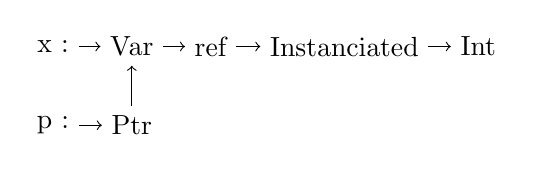
\begin{tikzpicture}
  \node               (var) {Var};
  \node[right of=var] (ref) {ref};
  \node[right of=ref, node distance=1.7cm] (u0) {Instanciated};
  \node[right of=u0, node distance=1.7cm] (ii) {Int};
  \node[below of=var] (ptr) {Ptr};
  \node[left of=var]  (x) {x :};
  \node[left of=ptr] (p) {p :};
  \draw[->] (x) -- (var);
  \draw[->] (p) -- (ptr);
  \draw[->] (ptr) -- (var);
  \draw[->] (var) -- (ref);
  \draw[->] (ref) -- (u0);
  \draw[->] (u0) -- (ii);
  \end{tikzpicture}
  }
  \subfloat[][]{
  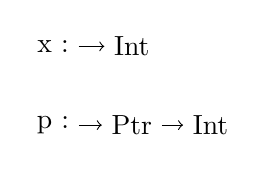
\begin{tikzpicture}
  \node               (var) {Int};
  \node[below of=var] (ptr) {Ptr};
  \node[left of=var]  (x) {x :};
  \node[left of=ptr] (p) {p :};
  \node[right of=ptr] (pi) {Int};
  \draw[->] (x) -- (var);
  \draw[->] (p) -- (ptr);
  \draw[->] (ptr) -- (pi);
  \end{tikzpicture}
  }

  \caption{Unification par partage}
  \label{fig:unifpartage}

\end{figure}
